%
%  HOW TO BUILD TOOLMAP DATAMODEL
%
%  Created by Lucien Schreiber on 2013-02-19.
%  Copyright (c) 2013. All rights reserved.
%

\documentclass[a4paper, 12pt]{article}
\usepackage{crealp-report}
\usepackage{upquote} %to force Latex not substitute ' by `
\usepackage{tocbibind}
\usepackage{mdwlist}
%\usepackage{natbib}

\begin{document}
\crealptitle {Tutorial} {How to create a ToolMap datamodel using TmDmCreator} {Lucien Schreiber} {lucien.schreiber@crealp.vs.ch}
\tableofcontents
\pagebreak

\section{Introduction}
This tutorial explains how to create a ToolMap project manually. This approach has the following advantages:
\begin{enumerate*}
  \item It ensures the IDs used
  \item It generates a multilingual model
  \item It allows better monitoring of model changes
\end{enumerate*}
The main disadvantage of this approach is the lack of user interface as well as the need for the user to have some knowledge of SQL. Finally, this approach has been developed to meet the need for rigor in the management of the Swiss geological data model.


\section{Conceptual Workflow}
The diagram shown in figure~\ref{fig:conceptual-workflow} illustrates the proposed workflow. User edits the user\_structure.sql and user\_content.txt files. These files as well as base\_structure.sql are used by the software TmDmCreator to produces either:
\begin{enumerate*}
  \item	a SQL file defining the project (output 1)
  \item	a ToolMap project (output 2)
\end{enumerate*}

\begin{figure} [htbp]
	\centering
    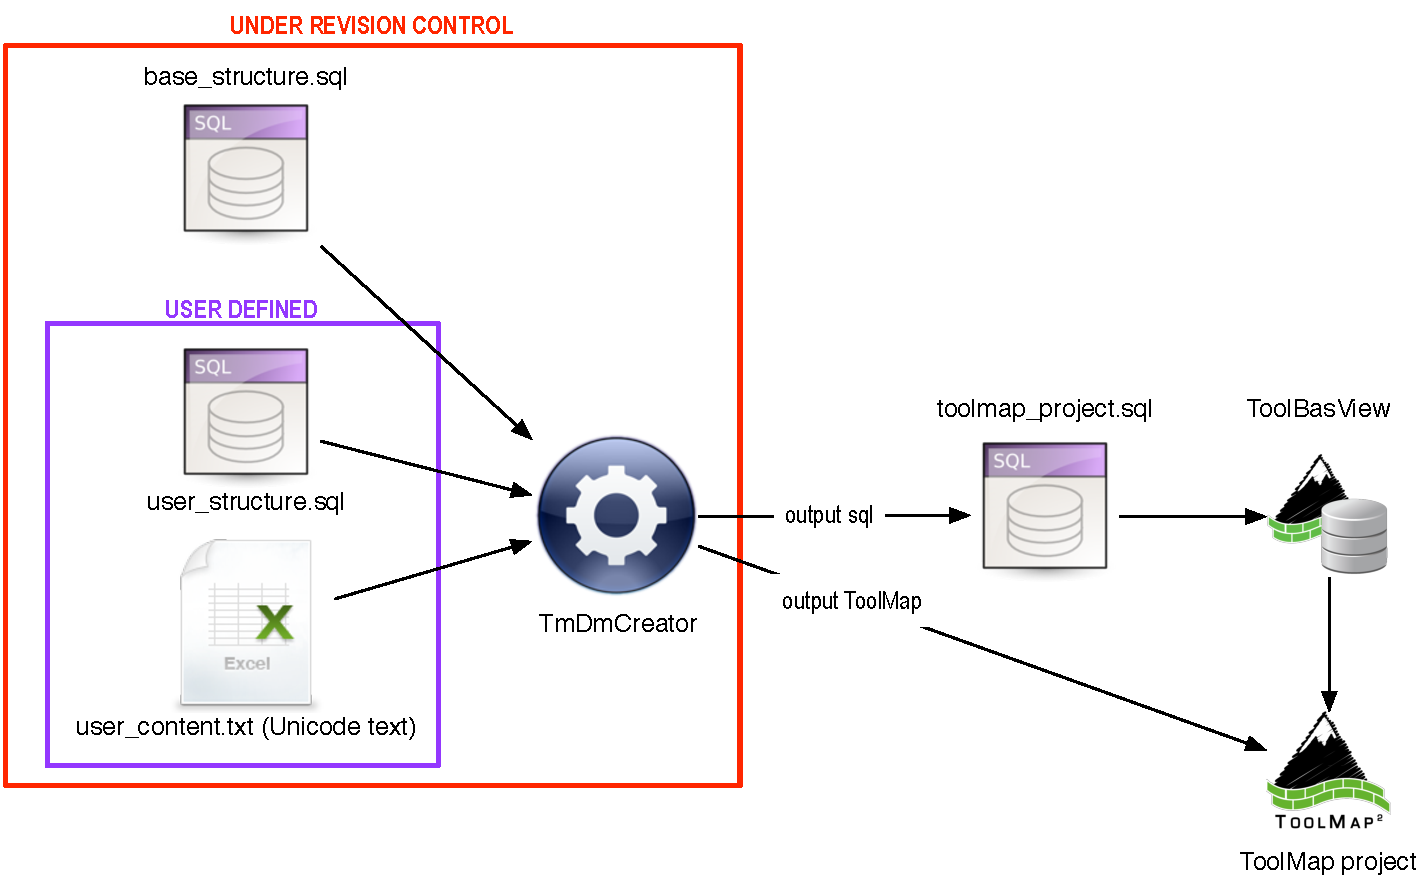
\includegraphics[width=1\textwidth]{img/workflow.pdf}
    \caption{Conceptual workflow}
    \label{fig:conceptual-workflow}
\end{figure}



\section{Data needed}
In order to produce a ToolMap project, TmDmCreator needs the following files:
%\begin{itemize}
    \begin{description*}
  \item[base\_structure.sql]\hfill \\ contains the necessary SQL code base for all ToolMap projects. This file should normally not be edited by users
  \item[user\_structure.sql]\hfill \\ contains the SQL structure describing the layers attributes
  \item[user\_content.txt]\hfill \\ Is a tabular file (editable in Excel for example) containing the definition of layers, objects, and attribute values.
\end{description*}
%\end{itemize}
The recommended way to work with user\_structure.sql and user\_content.txt is described below


\section{Preparing user data}

\subsection{Layers}
Open user\_content.txt using a spreadsheet and edit the thematic\_layers part. Each of the layers that we want to export should appear here. The structure is as follows (see figure~\ref{fig:layers}):
\begin{description*}
  \item [LAYER\_INDEX] unique identifier of the layer
  \item [TYPE\_CD] layer spatial type as follow
    \begin{description*}
      \item [0] = Line
      \item [1] = Point
      \item [2] = Polygon
    \end{description*}
  \item [LAYER\_NAME] the layer name. This name will be given to the SHP file when exporting
\end{description*}

\begin{figure} [hbp]
	\centering
    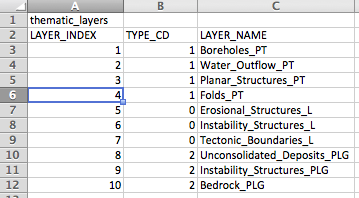
\includegraphics[width=.6\textwidth]{img/layers.png}
    \caption{List of layers as shown in user\_content.txt}
    \label{fig:layers}
\end{figure}

\subsection{Objects}

Edit the file user\_content.txt to add objects. They must have the following structure (See figure:~\ref{fig:objects}):
\begin{description*}
  \item [OBJECT\_ID] object unique ID.
  \item [OBJECT\_CD] object code, should not necessarily be unique
  \item [OBJECT\_TYPE\_CD] object spatial type, uses same values as those described above for TYPE\_CD in thematic\_layers
  \item [THEMATIC\_LAYERS\_LAYER\_INDEX] the index of the layer that the object refers to. The value 1 shown in the example (Figure 2) therefore relates to the theme Boreholes\_PT.
  \item [OBJECT\_DESC\_0,1,2,3,4,5] object description in up to 5 languages.
  \item [OBJECT\_ISFREQ] Set to 1 for frequent objects and 0 otherwise. This parameter is only taken into account for line type objects. Set to 0 for all point or polygon objects.
  \item [SYMBOL\_CD] leave empty
  \item [RANK] leave empty
  \item [REMARK] leave empty
\end{description*}

\begin{figure} [hbp]
	\centering
    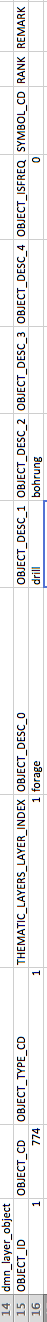
\includegraphics[height=.9\textheight]{img/objects.png}
    \caption{Objects structure as described in user\_content.txt}
    \label{fig:objects}
\end{figure}


\subsection{Attributes structure}
Edit the file user\_structure.sql with Notepad (or even better with Notepad + +). For each topic containing attributes, there must be a SQL code of the type:

\crealplisting{SQL}
\begin{lstlisting}
-- layer_at1 --
CREATE TABLE `layer_at1` (
  `OBJECT_ID` int(10) unsigned NOT NULL,
  PRIMARY KEY (`OBJECT_ID`),
  KEY `LAYER_ATX_FKIndex1` (`OBJECT_ID`)
) ENGINE=MyISAM DEFAULT CHARSET=utf8
\end{lstlisting}
This code is the basic template for creating an attribute table. The number after layer\_at (see line 2) indicates the layer index and refers to the LAYER\_INDEX column in user\_content.txt. In our example layer\_at1 describe the attributes for the layer Boreholes\_PT.
Below are described the five attributes that can be used as well as the corresponding SQL code
\begin{description*}
  \item [Enumeration] \hfill \\
    \crealplisting{SQL}
    \begin{lstlisting}
    `D_C_UNDERG` int(11) DEFAULT NULL COMMENT 'ENUMERATION',
    \end{lstlisting}
    If you add such fields, then you must also fill the list of supported values (see section~\ref{sec:attribute-values}).
  \item [Text] \hfill \\
    \begin{lstlisting}
    `DESCRIPT` varchar(255) DEFAULT NULL,
    \end{lstlisting}
    The number next to the keyword varchar indicates the maximum text length. 
  \item [Integer] \hfill \\
    \begin{lstlisting}
    `NUM_REF` int(11) DEFAULT NULL,       
    \end{lstlisting}
    There is no special option for integer fields
  \item [Float]  \hfill \\

    \begin{lstlisting}
    `TEMP` decimal(5,2) DEFAULT NULL,
    \end{lstlisting}
    The two digits next to the keyword decimal indicate the field precision and scale. In this example, 5 is the precision and 2 is the scale. The precision represents the number of significant digits that are stored for values, and the scale represents the number of digits that can be stored following the decimal point. In this case, values that can be stored range from -999.99 to 999.99.
  \item [Date] \hfill \\

    \begin{lstlisting}
    `REF_DATE` date DEFAULT NULL,
    \end{lstlisting}
    There is no special option for date fields
\end{description*}


\subsection{Value domain of the attributes}
\label{sec:attribute-values}



\end{document}
